\section{10 класс}

\AddProb Радиус рукоятки колодезного ворота в $3$ раза больше радиуса вала, на который наматывается трос. 
Какова линейная скорость конца рукоятки, если ведро с глубины $10$~м поднимается за $20$~с.

\AddProb Оцените, до какой температуры нужно нагреть воздух внутри оболочки воздушного шара объемом 500 м$^3$, 
чтобы он мог поднять человека массой 70~кг? Масса оболочки шара равна 30~кг.

\AddProb Гиря массой $m$ падает на чашку пружинных весов с высоты $H$ и испытывает абсолютно упругий удар. 
На какую величину $h$ сожмется пружина весов после удара, если масса чашки равна $M$, а коэффициент жесткости пружины равен $k$?

%Задача 118, молекулярка, ЗСЭ
\begin{wrapfigure}{r}{3cm}
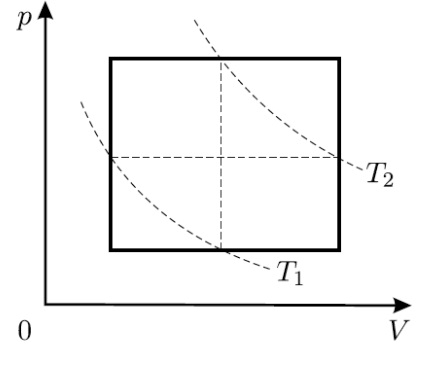
\includegraphics[scale=0.25]{0904LawOfConservationOfEnergyEfficiency.jpg}
\end{wrapfigure}

\AddProb Найдите КПД тепловой машины, цикл которой состоит из двух изохор и двух изобар, а рабочим телом является идеальный одноатомный газ. 
Середины нижней изобары и левой изохоры лежат на изотерме, соответствующей температуре $T_1$, 
а середины верхней изобары и правой изохоры -- на изотерме, соответствующей температуре $T_2$.



\section{11 класс}

\AddProb По первоначальным предположениям Бора, электрон в водородном атоме движется по круговой орбите. 
С какой скоростью $v$ должен двигаться такой электрон, если заряд электрона $q_1\,=\,-1.6\cdot~10^{-19}$~Кл, 
заряд ядра $q_2\,=\,1.6\cdot~10^{-19}$~Кл, радиус орбиты можно принять равным $r\,=\,0.5\cdot 10^{-10}$~м, масса электрона $m\,=\,9.1\cdot 10^{-31}$~кг.

\AddProb Ящик, имеющий форму куба с длинной ребра $L$, находится на горизонтальной поверхности. 
При каких значениях коэффициента трения между ящиком и поверхностью работа при перемещении ящика волоком на расстояние $L$ будет больше, 
чем работа при кантовании (опрокидывании через ребро)?

% Задача 159, электричество, ЭМИ
\begin{wrapfigure}{r}{5cm}
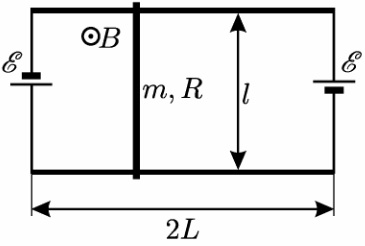
\includegraphics[scale=0.5]{1214EMIRailsAndBridge.jpg}
\end{wrapfigure}

\AddProb Параллельные рельсы длиной $2L$ закреплены на горизонтальной плоскости на расстоянии $l$ друг от друга. 
К их концам подсоединены две одинаковые батареи с ЭДС {\Large $\varepsilon$}. На рельсах лежит перемычка массы $m$, 
которая может поступательно скользить вдоль них. Вся система помещена в однородное вертикальное магнитное поле с индукцией $B$. 
Считая, что сопротивление перемычки равно $R$, а сопротивление единицы длины каждого из рельсов равно $\rho$, найдите период малых колебаний, 
возникающих при смещении перемычки от положения равновесия, пренебрегая затуханием, внутренним сопротивлением источников, 
сопротивлением контактов, а также индуктивностью цепи.

\AddProb Горизонтальный закрытый теплоизолированный цилиндр разделен на две части тонким теплопроводящим поршнем, 
который прикреплен пружиной к одной из торцевых стенок цилиндра. Слева и справа от поршня находятся по $\nu$ молей идеального одноатомного газа. 
Начальная температура системы $T$, длина цилиндра $2L$, собственная длина пружины $L/2$, удлинение пружины в состоянии равновесия равно $L/4$. 
В поршне проделали отверстие. Как изменится температура этой системы после установления нового равновесия? 
Теплоемкостями цилиндра, поршня и пружины пренебречь, трения нет.